% Options for packages loaded elsewhere
\PassOptionsToPackage{unicode}{hyperref}
\PassOptionsToPackage{hyphens}{url}
%
\documentclass[
]{article}
\usepackage{amsmath,amssymb}
\usepackage{lmodern}
\usepackage{setspace}
\usepackage{ifxetex,ifluatex}
\ifnum 0\ifxetex 1\fi\ifluatex 1\fi=0 % if pdftex
  \usepackage[T1]{fontenc}
  \usepackage[utf8]{inputenc}
  \usepackage{textcomp} % provide euro and other symbols
\else % if luatex or xetex
  \usepackage{unicode-math}
  \defaultfontfeatures{Scale=MatchLowercase}
  \defaultfontfeatures[\rmfamily]{Ligatures=TeX,Scale=1}
\fi
% Use upquote if available, for straight quotes in verbatim environments
\IfFileExists{upquote.sty}{\usepackage{upquote}}{}
\IfFileExists{microtype.sty}{% use microtype if available
  \usepackage[]{microtype}
  \UseMicrotypeSet[protrusion]{basicmath} % disable protrusion for tt fonts
}{}
\makeatletter
\@ifundefined{KOMAClassName}{% if non-KOMA class
  \IfFileExists{parskip.sty}{%
    \usepackage{parskip}
  }{% else
    \setlength{\parindent}{0pt}
    \setlength{\parskip}{6pt plus 2pt minus 1pt}}
}{% if KOMA class
  \KOMAoptions{parskip=half}}
\makeatother
\usepackage{xcolor}
\IfFileExists{xurl.sty}{\usepackage{xurl}}{} % add URL line breaks if available
\IfFileExists{bookmark.sty}{\usepackage{bookmark}}{\usepackage{hyperref}}
\hypersetup{
  pdftitle={Bayesian Cumulative Probability Models for Continuous and Mixed Outcomes},
  pdfauthor={Nathan T. James, Frank E. Harrell Jr., Bryan E. Shepherd},
  hidelinks}
\urlstyle{same} % disable monospaced font for URLs
\usepackage{longtable,booktabs,array}
\usepackage{calc} % for calculating minipage widths
% Correct order of tables after \paragraph or \subparagraph
\usepackage{etoolbox}
\makeatletter
\patchcmd\longtable{\par}{\if@noskipsec\mbox{}\fi\par}{}{}
\makeatother
% Allow footnotes in longtable head/foot
\IfFileExists{footnotehyper.sty}{\usepackage{footnotehyper}}{\usepackage{footnote}}
\makesavenoteenv{longtable}
\usepackage{graphicx}
\makeatletter
\def\maxwidth{\ifdim\Gin@nat@width>\linewidth\linewidth\else\Gin@nat@width\fi}
\def\maxheight{\ifdim\Gin@nat@height>\textheight\textheight\else\Gin@nat@height\fi}
\makeatother
% Scale images if necessary, so that they will not overflow the page
% margins by default, and it is still possible to overwrite the defaults
% using explicit options in \includegraphics[width, height, ...]{}
\setkeys{Gin}{width=\maxwidth,height=\maxheight,keepaspectratio}
% Set default figure placement to htbp
\makeatletter
\def\fps@figure{htbp}
\makeatother
\setlength{\emergencystretch}{3em} % prevent overfull lines
\providecommand{\tightlist}{%
  \setlength{\itemsep}{0pt}\setlength{\parskip}{0pt}}
\setcounter{secnumdepth}{-\maxdimen} % remove section numbering
\usepackage{titlesec}
\usepackage{booktabs}
\usepackage{longtable}
\usepackage{array}
\usepackage{multirow}
\usepackage{wrapfig}
\usepackage{float}
\usepackage{colortbl}
\usepackage{pdflscape}
\usepackage{tabu}
\usepackage{threeparttable}
\usepackage{threeparttablex}
\usepackage[normalem]{ulem}
\usepackage{makecell}

\special{papersize=8.5in,11in}
\setlength{\pdfpageheight}{\paperheight}
\setlength{\pdfpagewidth}{\paperwidth}

% reduce spacing around gather environments
%\abovedisplayshortskip=0pt
%\belowdisplayshortskip=0pt
%\abovedisplayskip=0pt
%\belowdisplayskip=0pt

\setlength{\abovedisplayshortskip}{0pt}
\setlength{\belowdisplayshortskip}{0pt}
\setlength{\abovedisplayskip}{0pt}
\setlength{\belowdisplayskip}{0pt}

\setlength{\textwidth}{7in}
\setlength{\textheight}{9.75in}
\setlength{\oddsidemargin}{-.25in}
\setlength{\parskip}{0.15in}
\setlength{\topmargin}{0in}
\setlength{\headheight}{-.5in}
\setlength{\headsep}{0in}
\setlength\parindent{0pt}

%\titleformat{\chapter}
%  {\normalfont\LARGE\bfseries}{\thechapter}{1em}{}
%\titlespacing*{\chapter}{0pt}{3.5ex plus 1ex minus .2ex}{2.3ex plus .2ex}

\newcommand{\beginsupplement}{
  \setcounter{table}{0}
  \renewcommand{\thetable}{S\arabic{table}}
  \setcounter{figure}{0}
  \renewcommand{\thefigure}{S\arabic{figure}}
}
\ifluatex
  \usepackage{selnolig}  % disable illegal ligatures
\fi
\newlength{\cslhangindent}
\setlength{\cslhangindent}{1.5em}
\newlength{\csllabelwidth}
\setlength{\csllabelwidth}{3em}
\newenvironment{CSLReferences}[2] % #1 hanging-ident, #2 entry spacing
 {% don't indent paragraphs
  \setlength{\parindent}{0pt}
  % turn on hanging indent if param 1 is 1
  \ifodd #1 \everypar{\setlength{\hangindent}{\cslhangindent}}\ignorespaces\fi
  % set entry spacing
  \ifnum #2 > 0
  \setlength{\parskip}{#2\baselineskip}
  \fi
 }%
 {}
\usepackage{calc}
\newcommand{\CSLBlock}[1]{#1\hfill\break}
\newcommand{\CSLLeftMargin}[1]{\parbox[t]{\csllabelwidth}{#1}}
\newcommand{\CSLRightInline}[1]{\parbox[t]{\linewidth - \csllabelwidth}{#1}\break}
\newcommand{\CSLIndent}[1]{\hspace{\cslhangindent}#1}


\begin{document}
\beginsupplement

\setstretch{1.5}

\subsection{Supplemental Material}

% Figure S1
\begin{figure}
{\centering 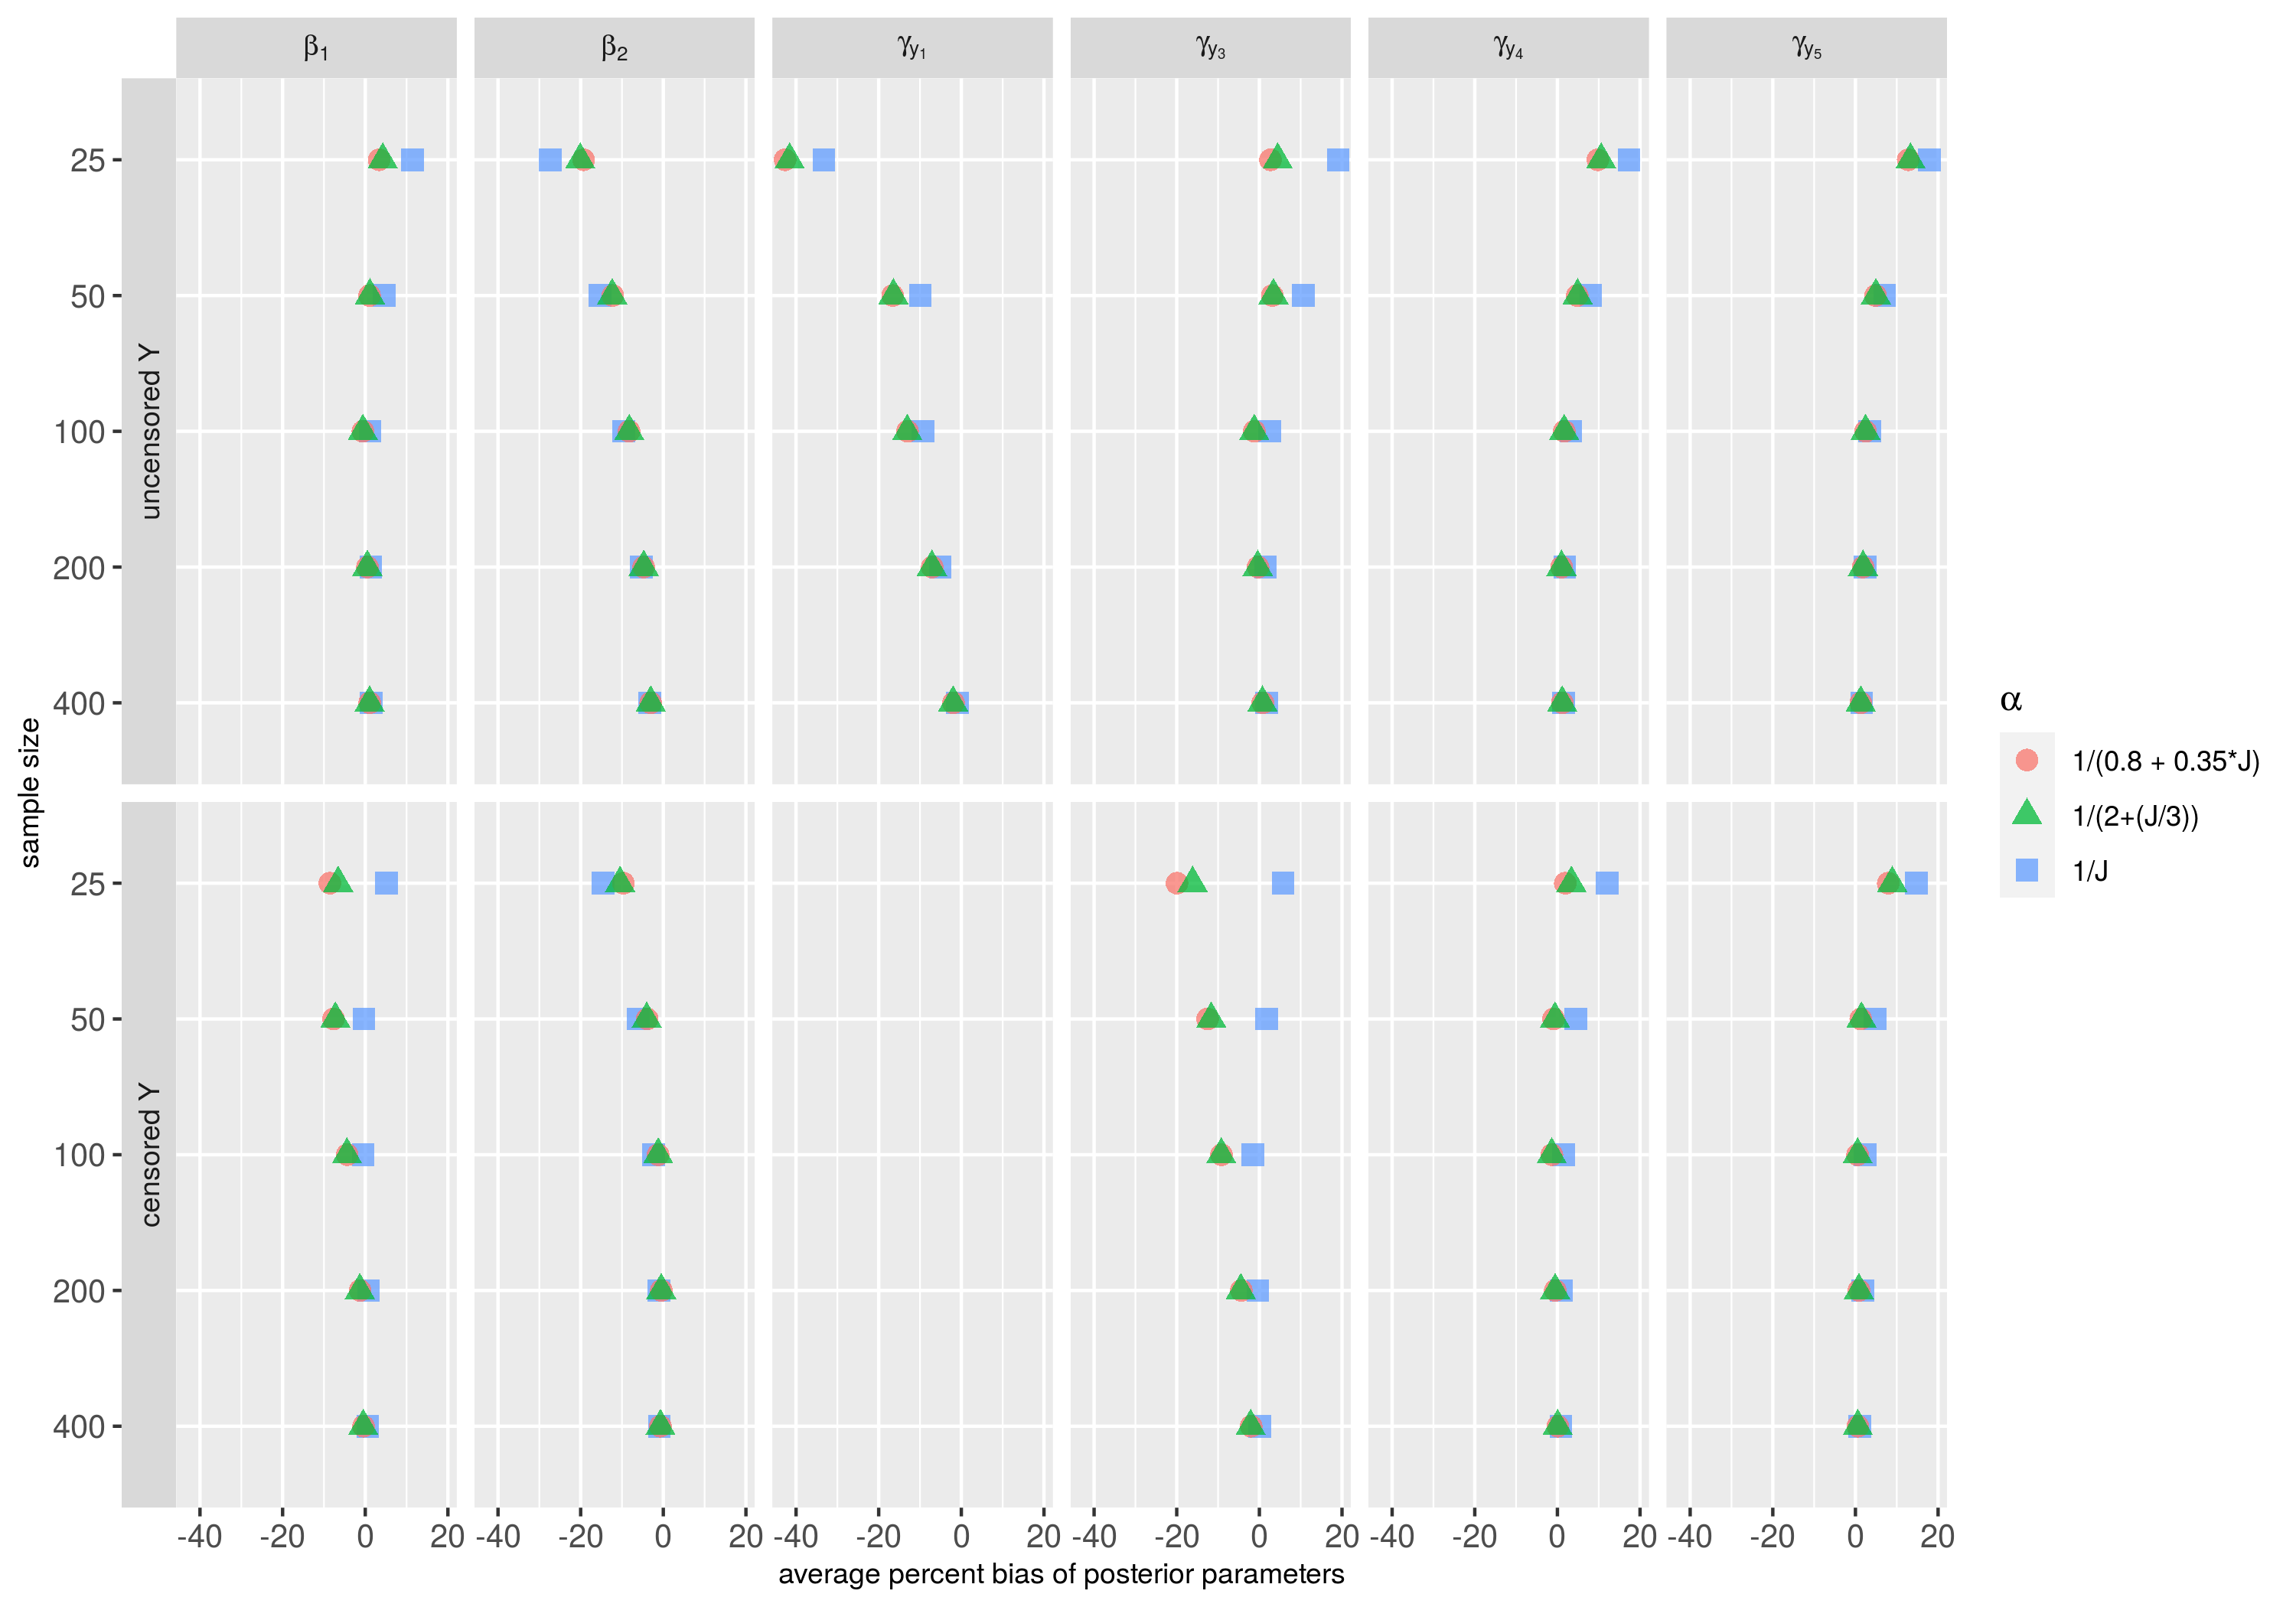
\includegraphics[width=0.75\linewidth]{fig/sim_d_pars} 

}
\caption{Bias in parameters for simulations using loglog link}
\end{figure}

% Figure S2
\begin{figure}
{\centering 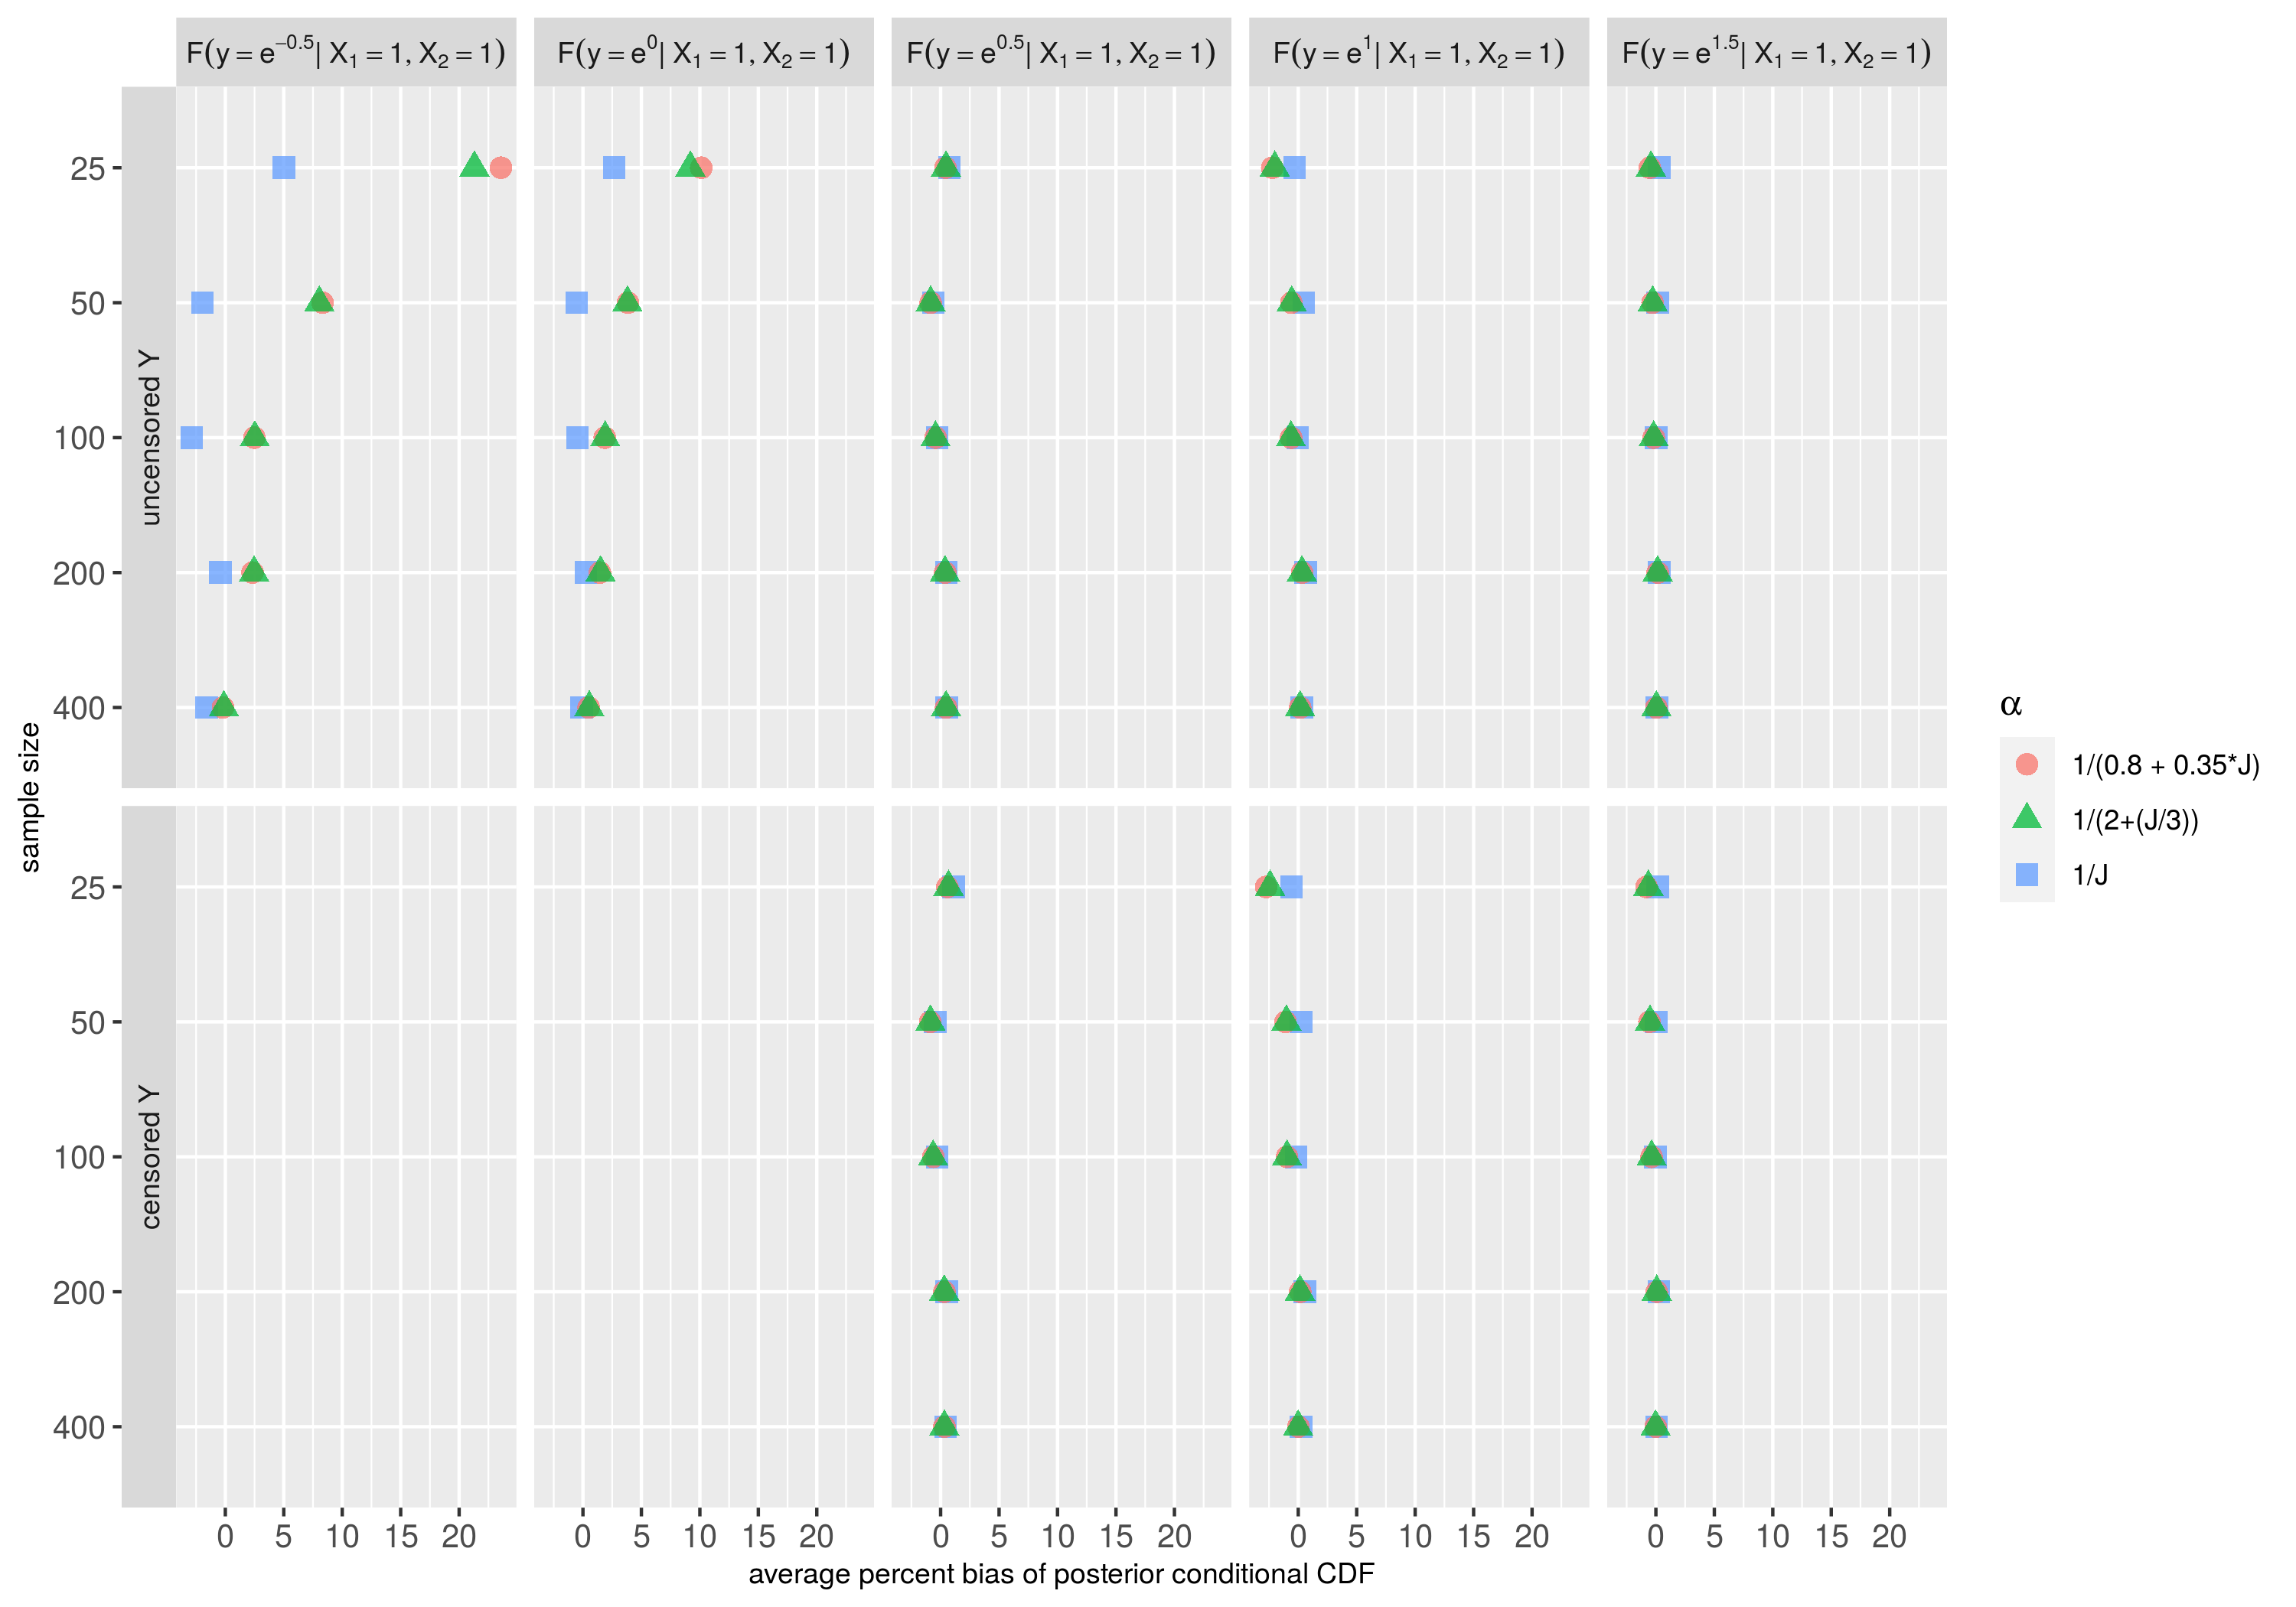
\includegraphics[width=0.75\linewidth]{fig/sim_c_cdf} 

}
\caption{Percent bias in conditional CDF for simulations using logit link}
\end{figure}

% Figure S3
\begin{figure}
{\centering 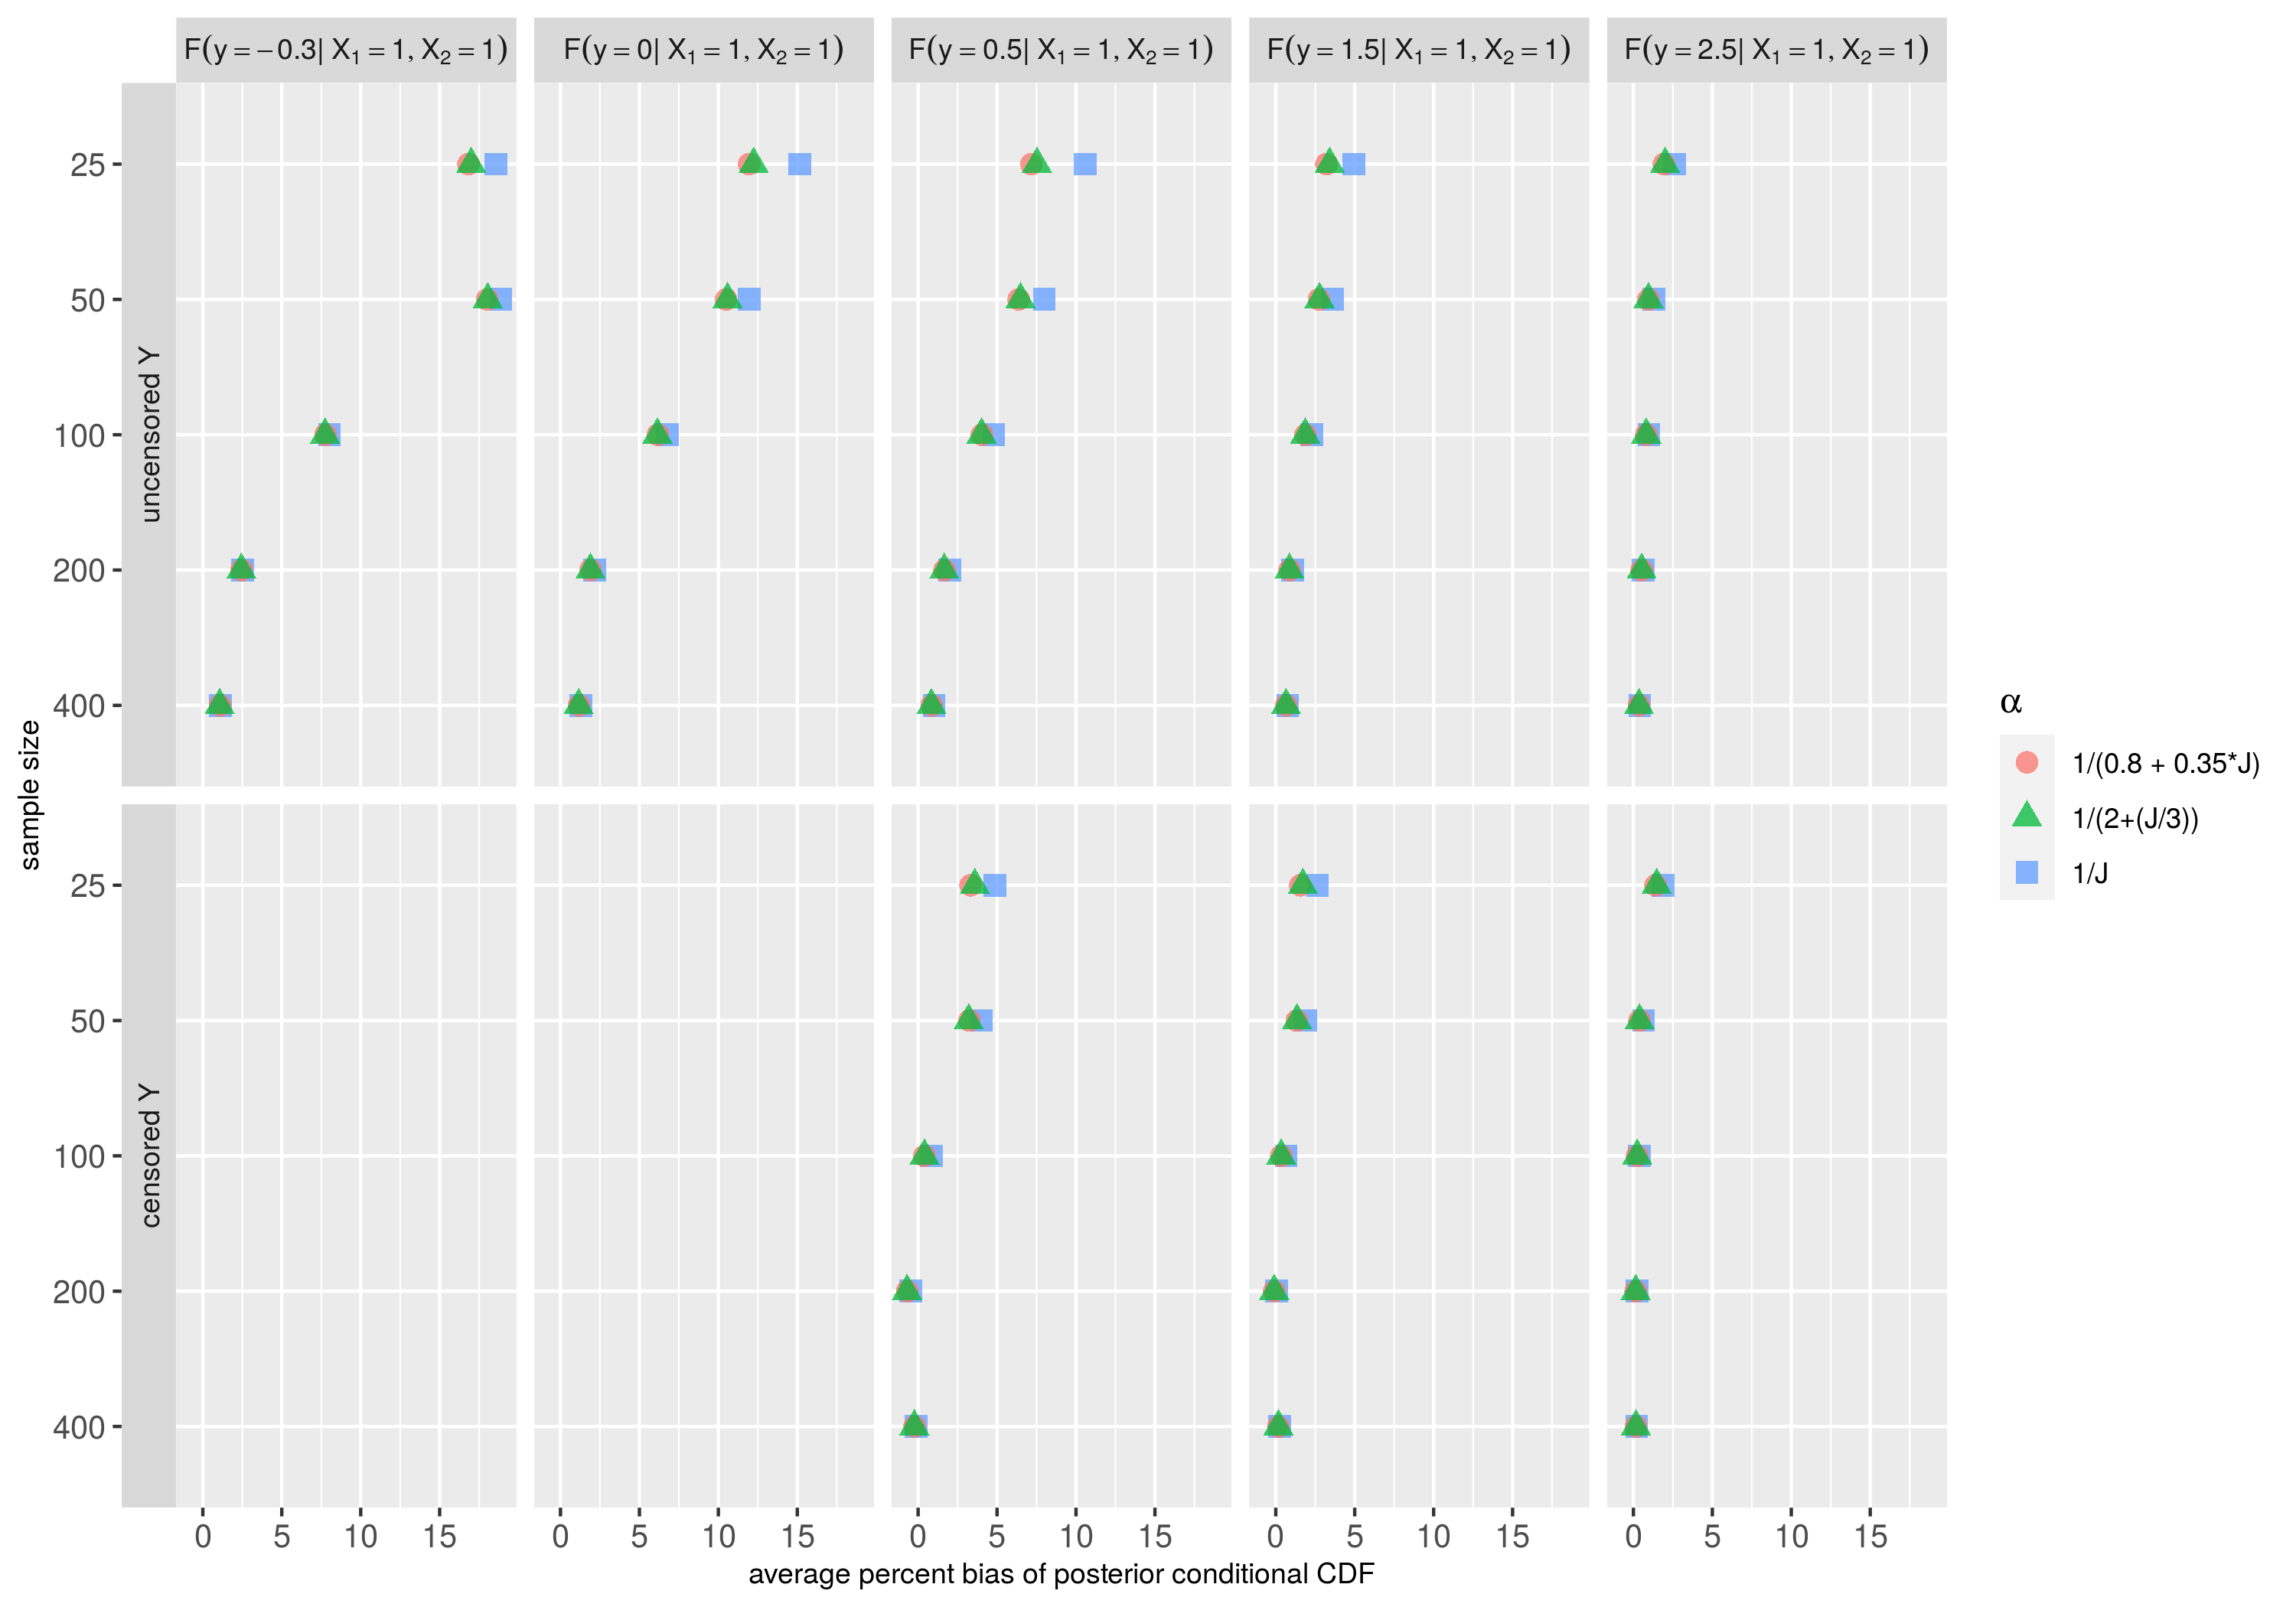
\includegraphics[width=0.75\linewidth]{fig/sim_d_cdf} 

}
\caption{Percent bias in conditional CDF for simulations using loglog link}
\end{figure}

% Figure S4
\begin{figure}
{\centering 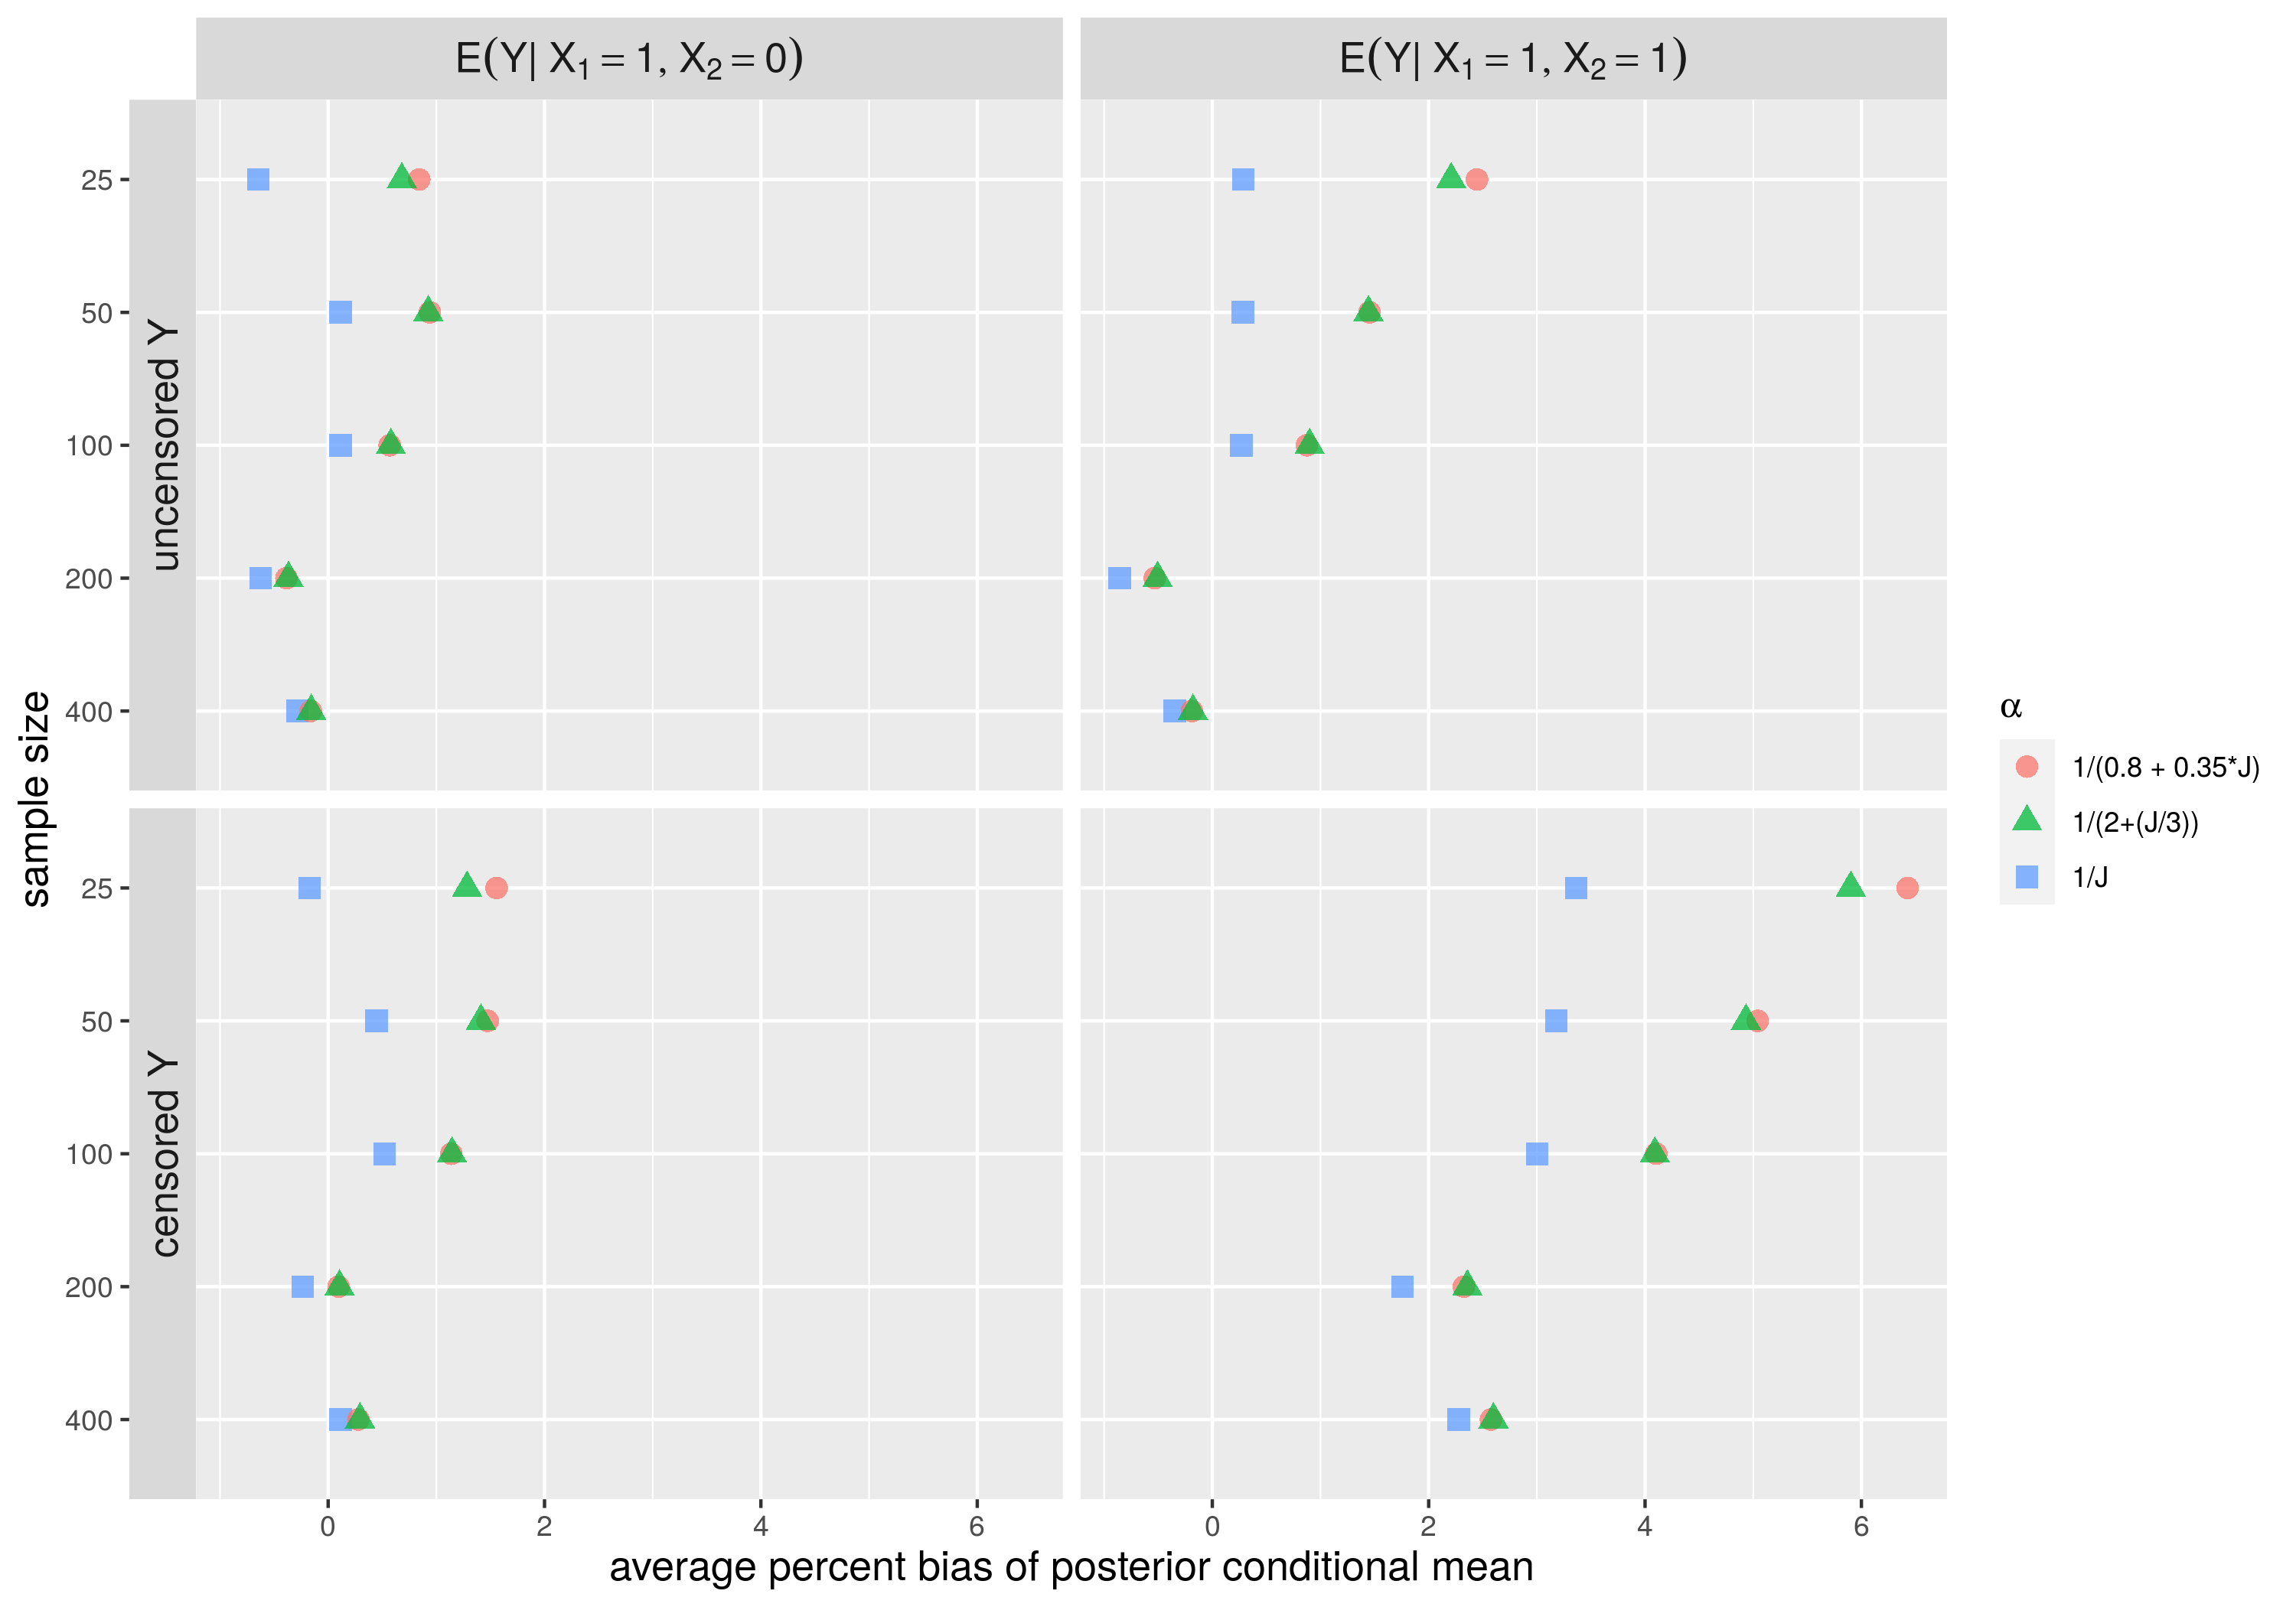
\includegraphics[width=0.75\linewidth]{fig/sim_c_mn} 

}
\caption{Percent bias in conditional mean for simulations using logit link}
\end{figure}

% Figure S5
\begin{figure}
{\centering 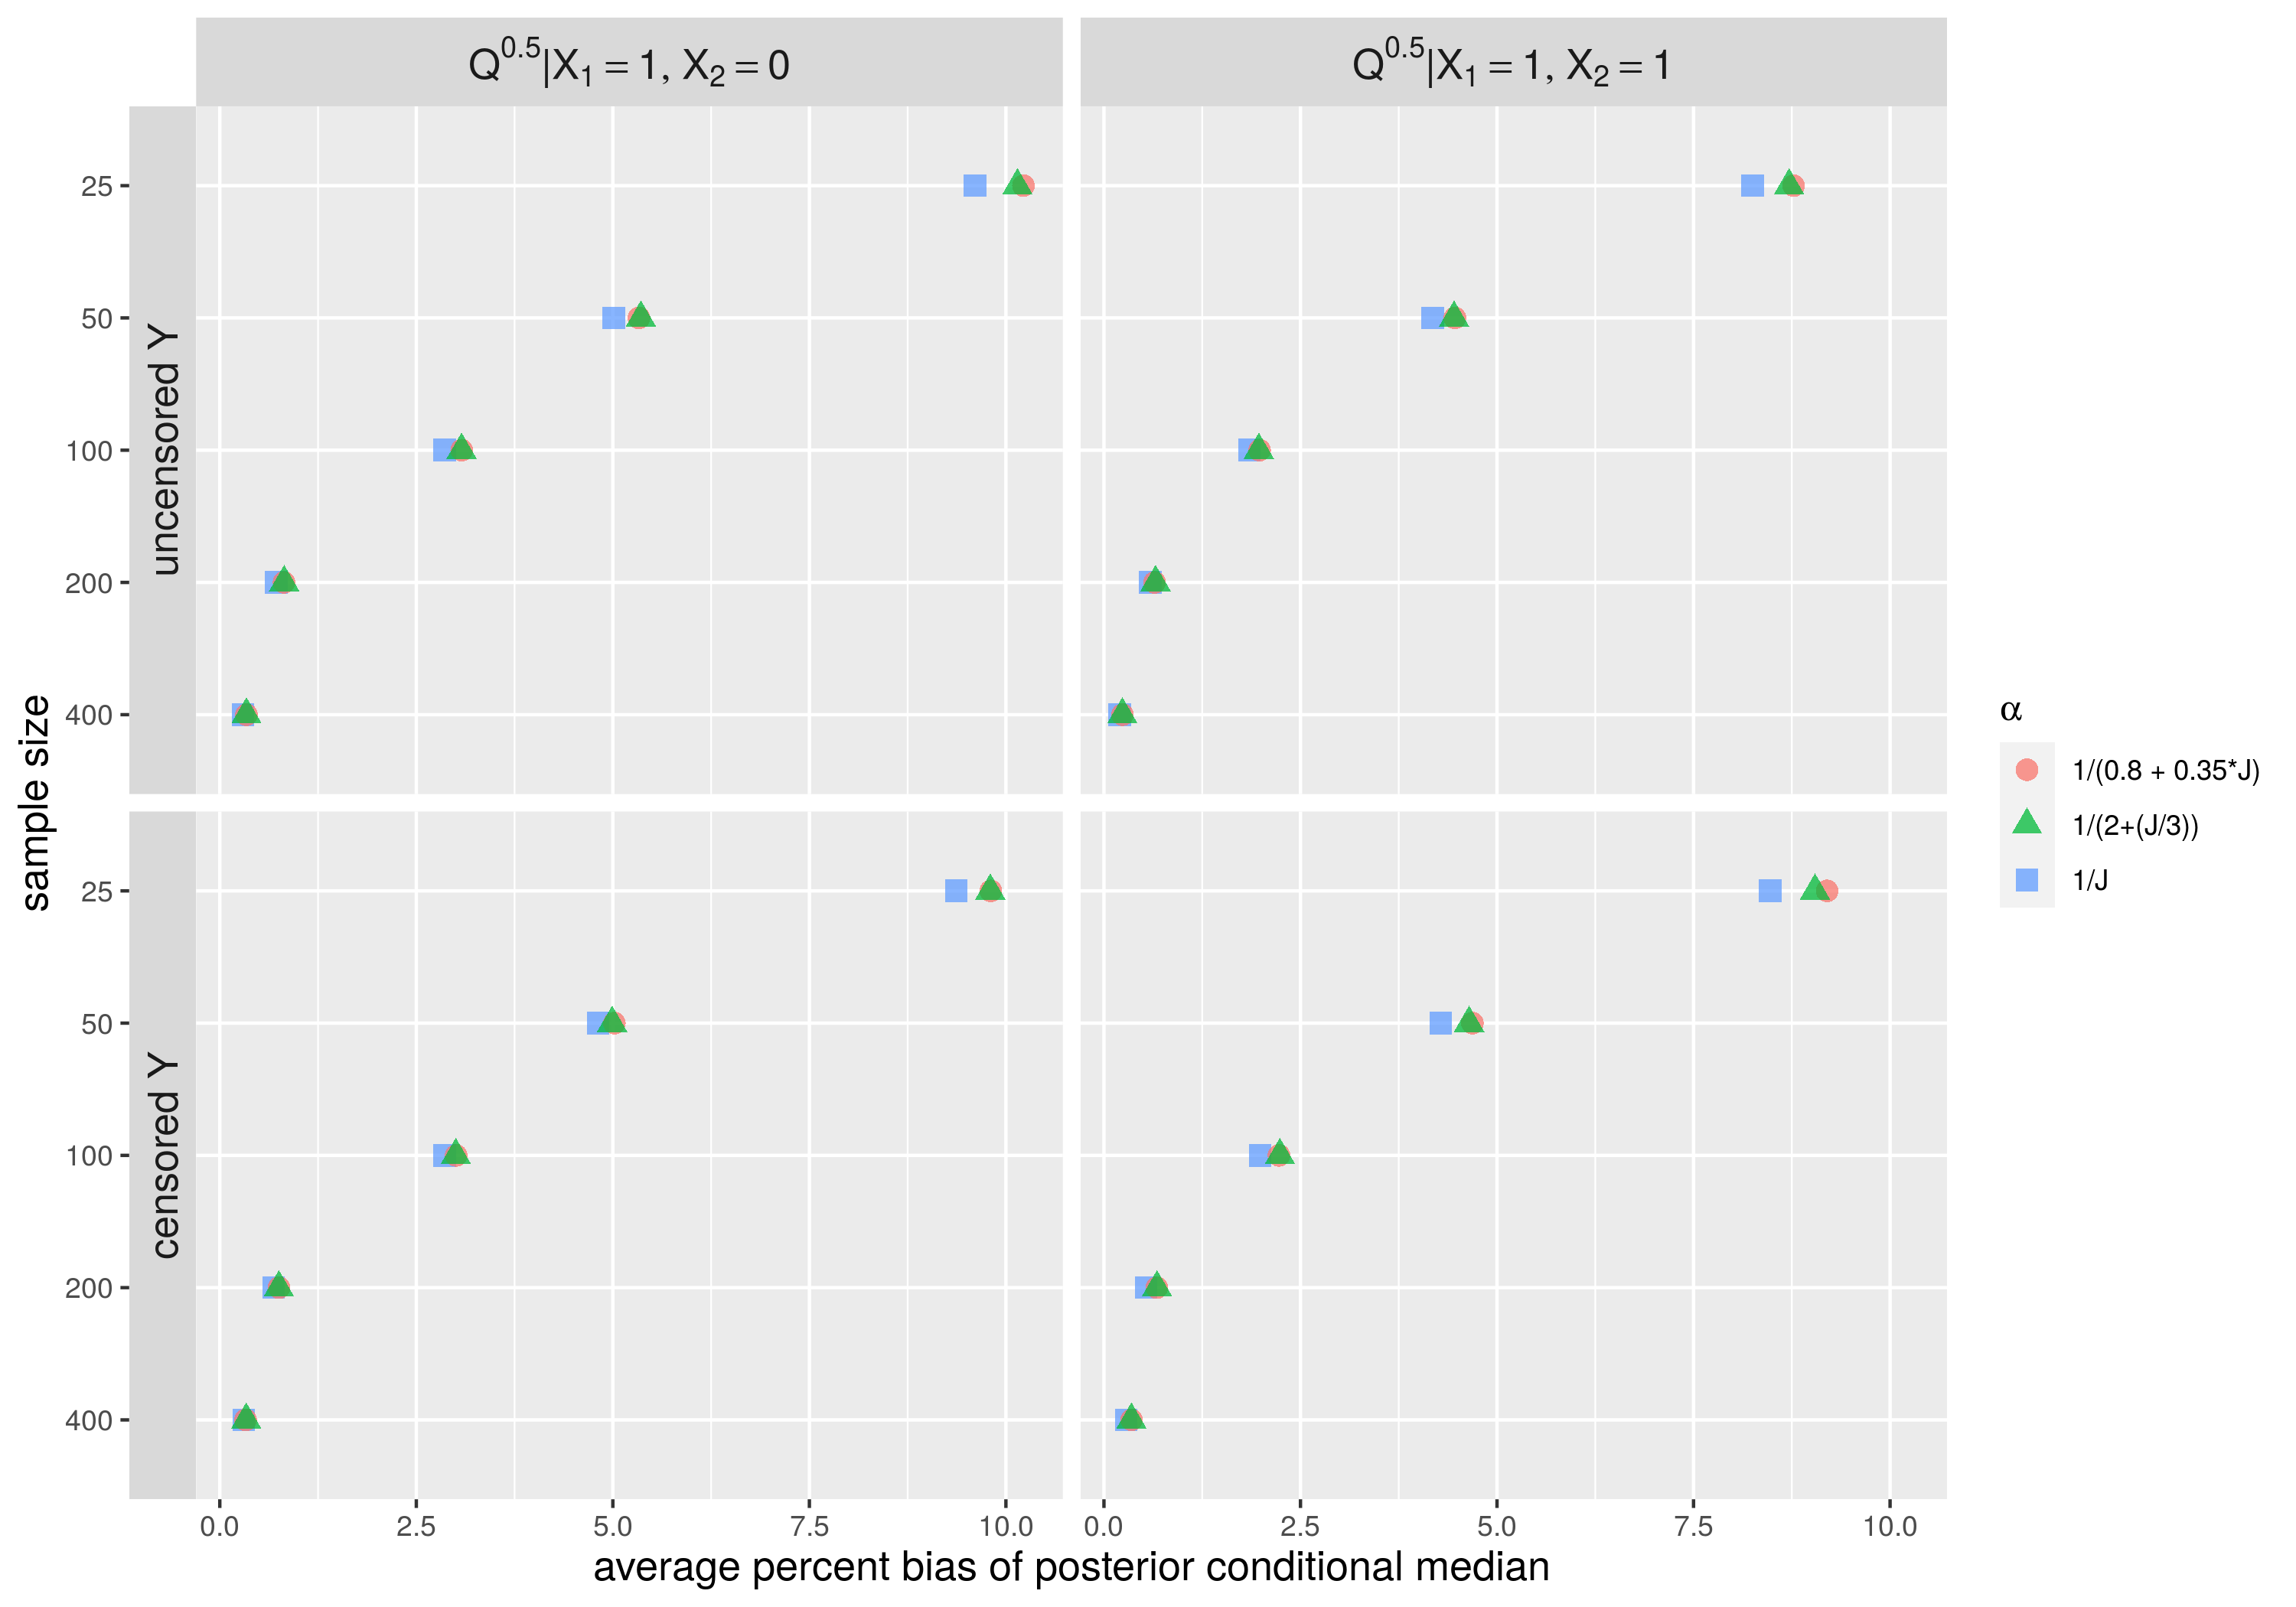
\includegraphics[width=0.75\linewidth]{fig/sim_c_med} 

}
\caption{Percent bias in conditional median for simulations using logit link}
\end{figure}

% Figure S6
\begin{figure}
{\centering 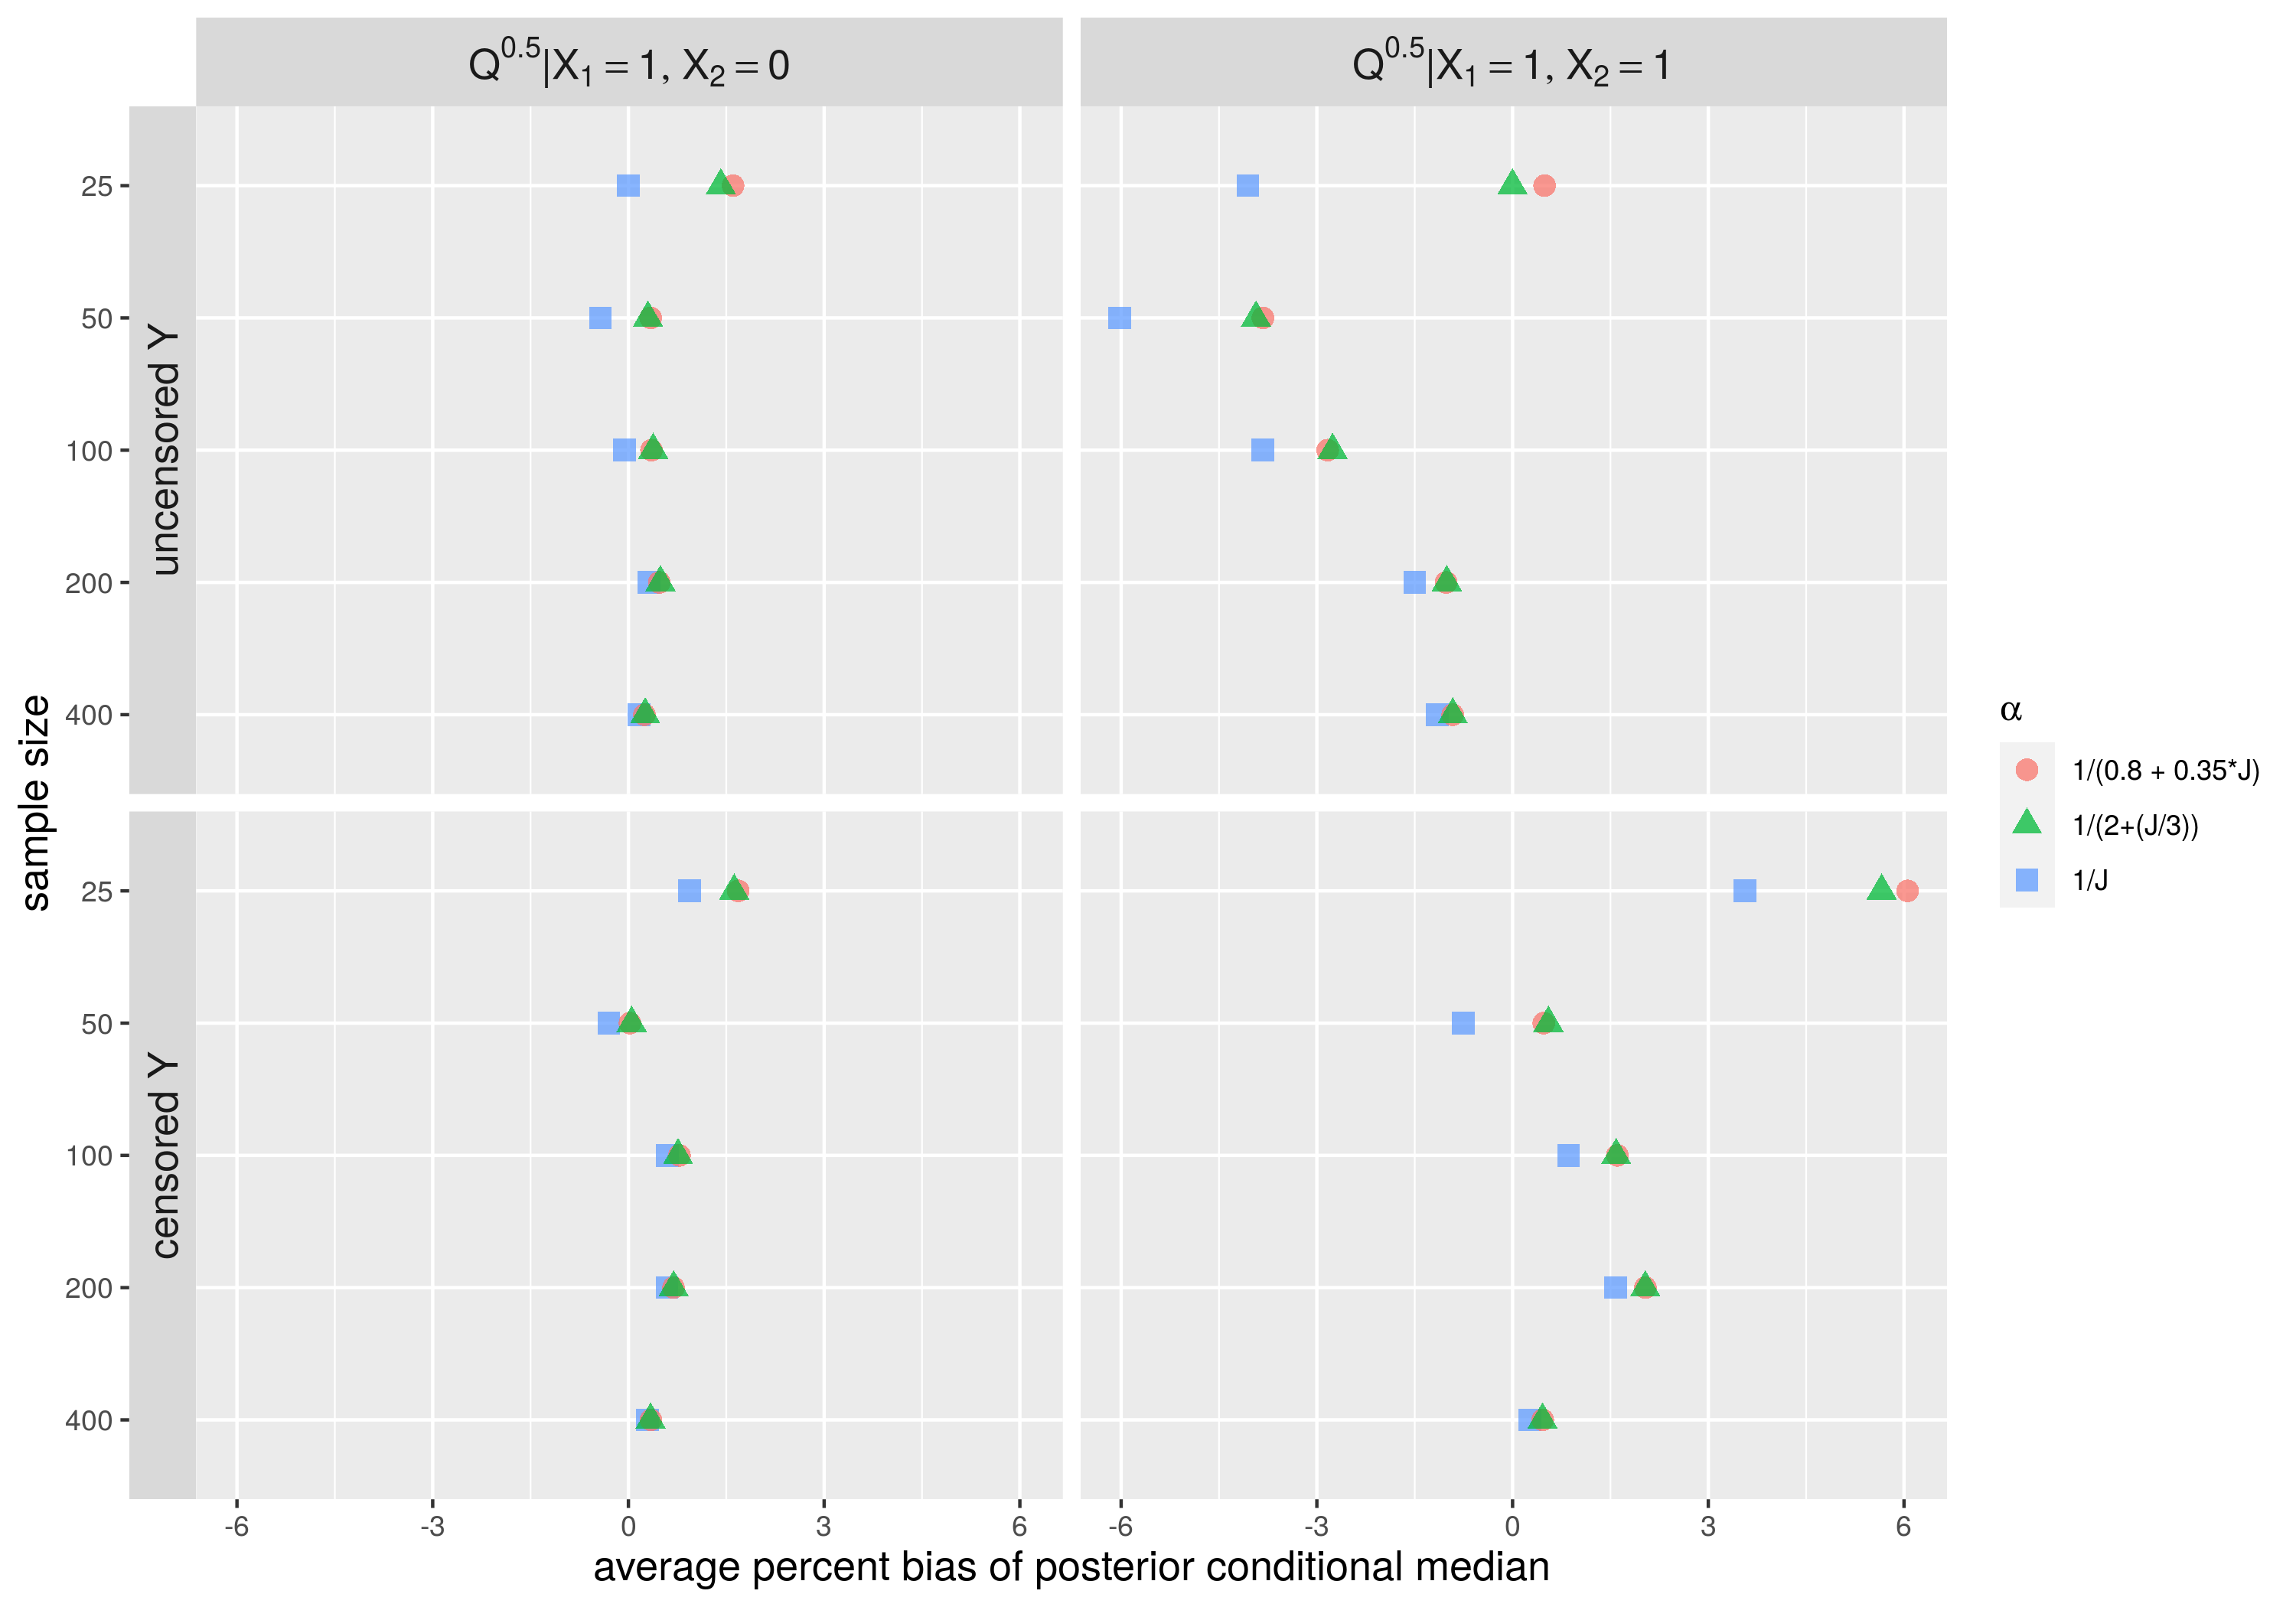
\includegraphics[width=0.75\linewidth]{fig/sim_d_med} 

}
\caption{Percent bias in conditional median for simulations using loglog link}
\end{figure}

% Figure S7
\begin{figure}
{\centering 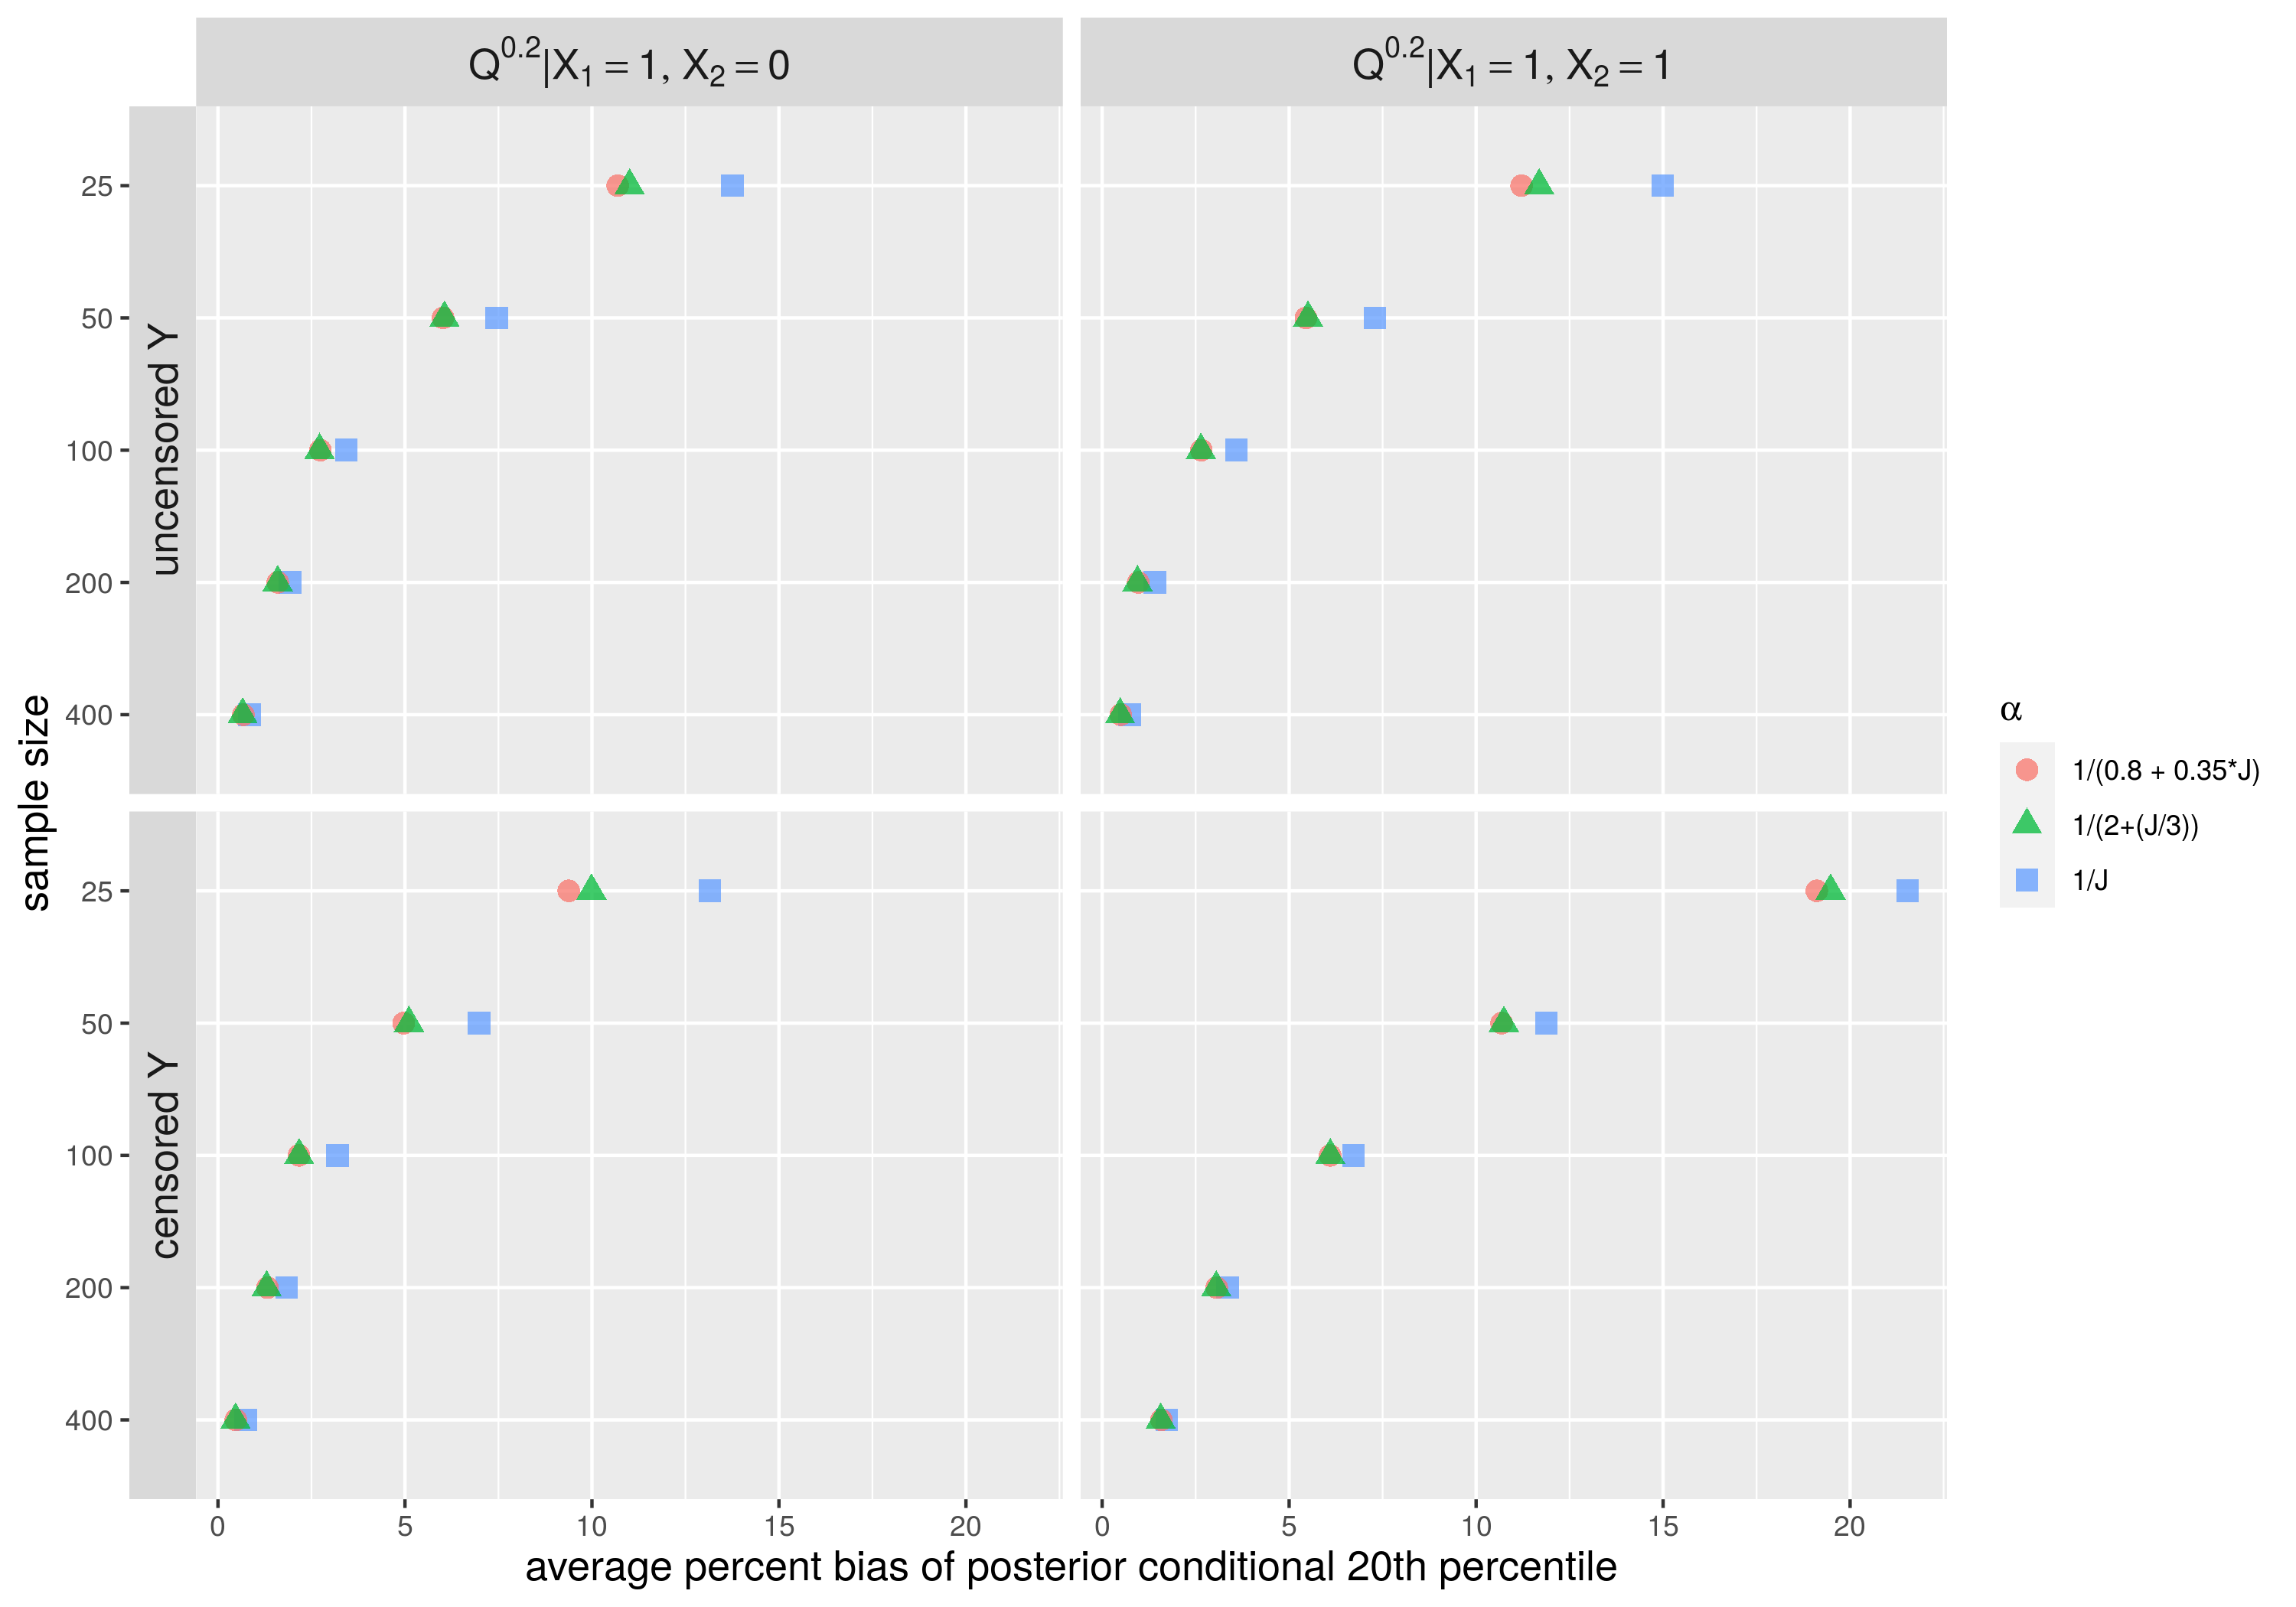
\includegraphics[width=0.75\linewidth]{fig/sim_c_q20} 

}
\caption{Bias in conditional 20th percentile for simulations using logit link}
\end{figure}

% Figure S8
\begin{figure}
{\centering 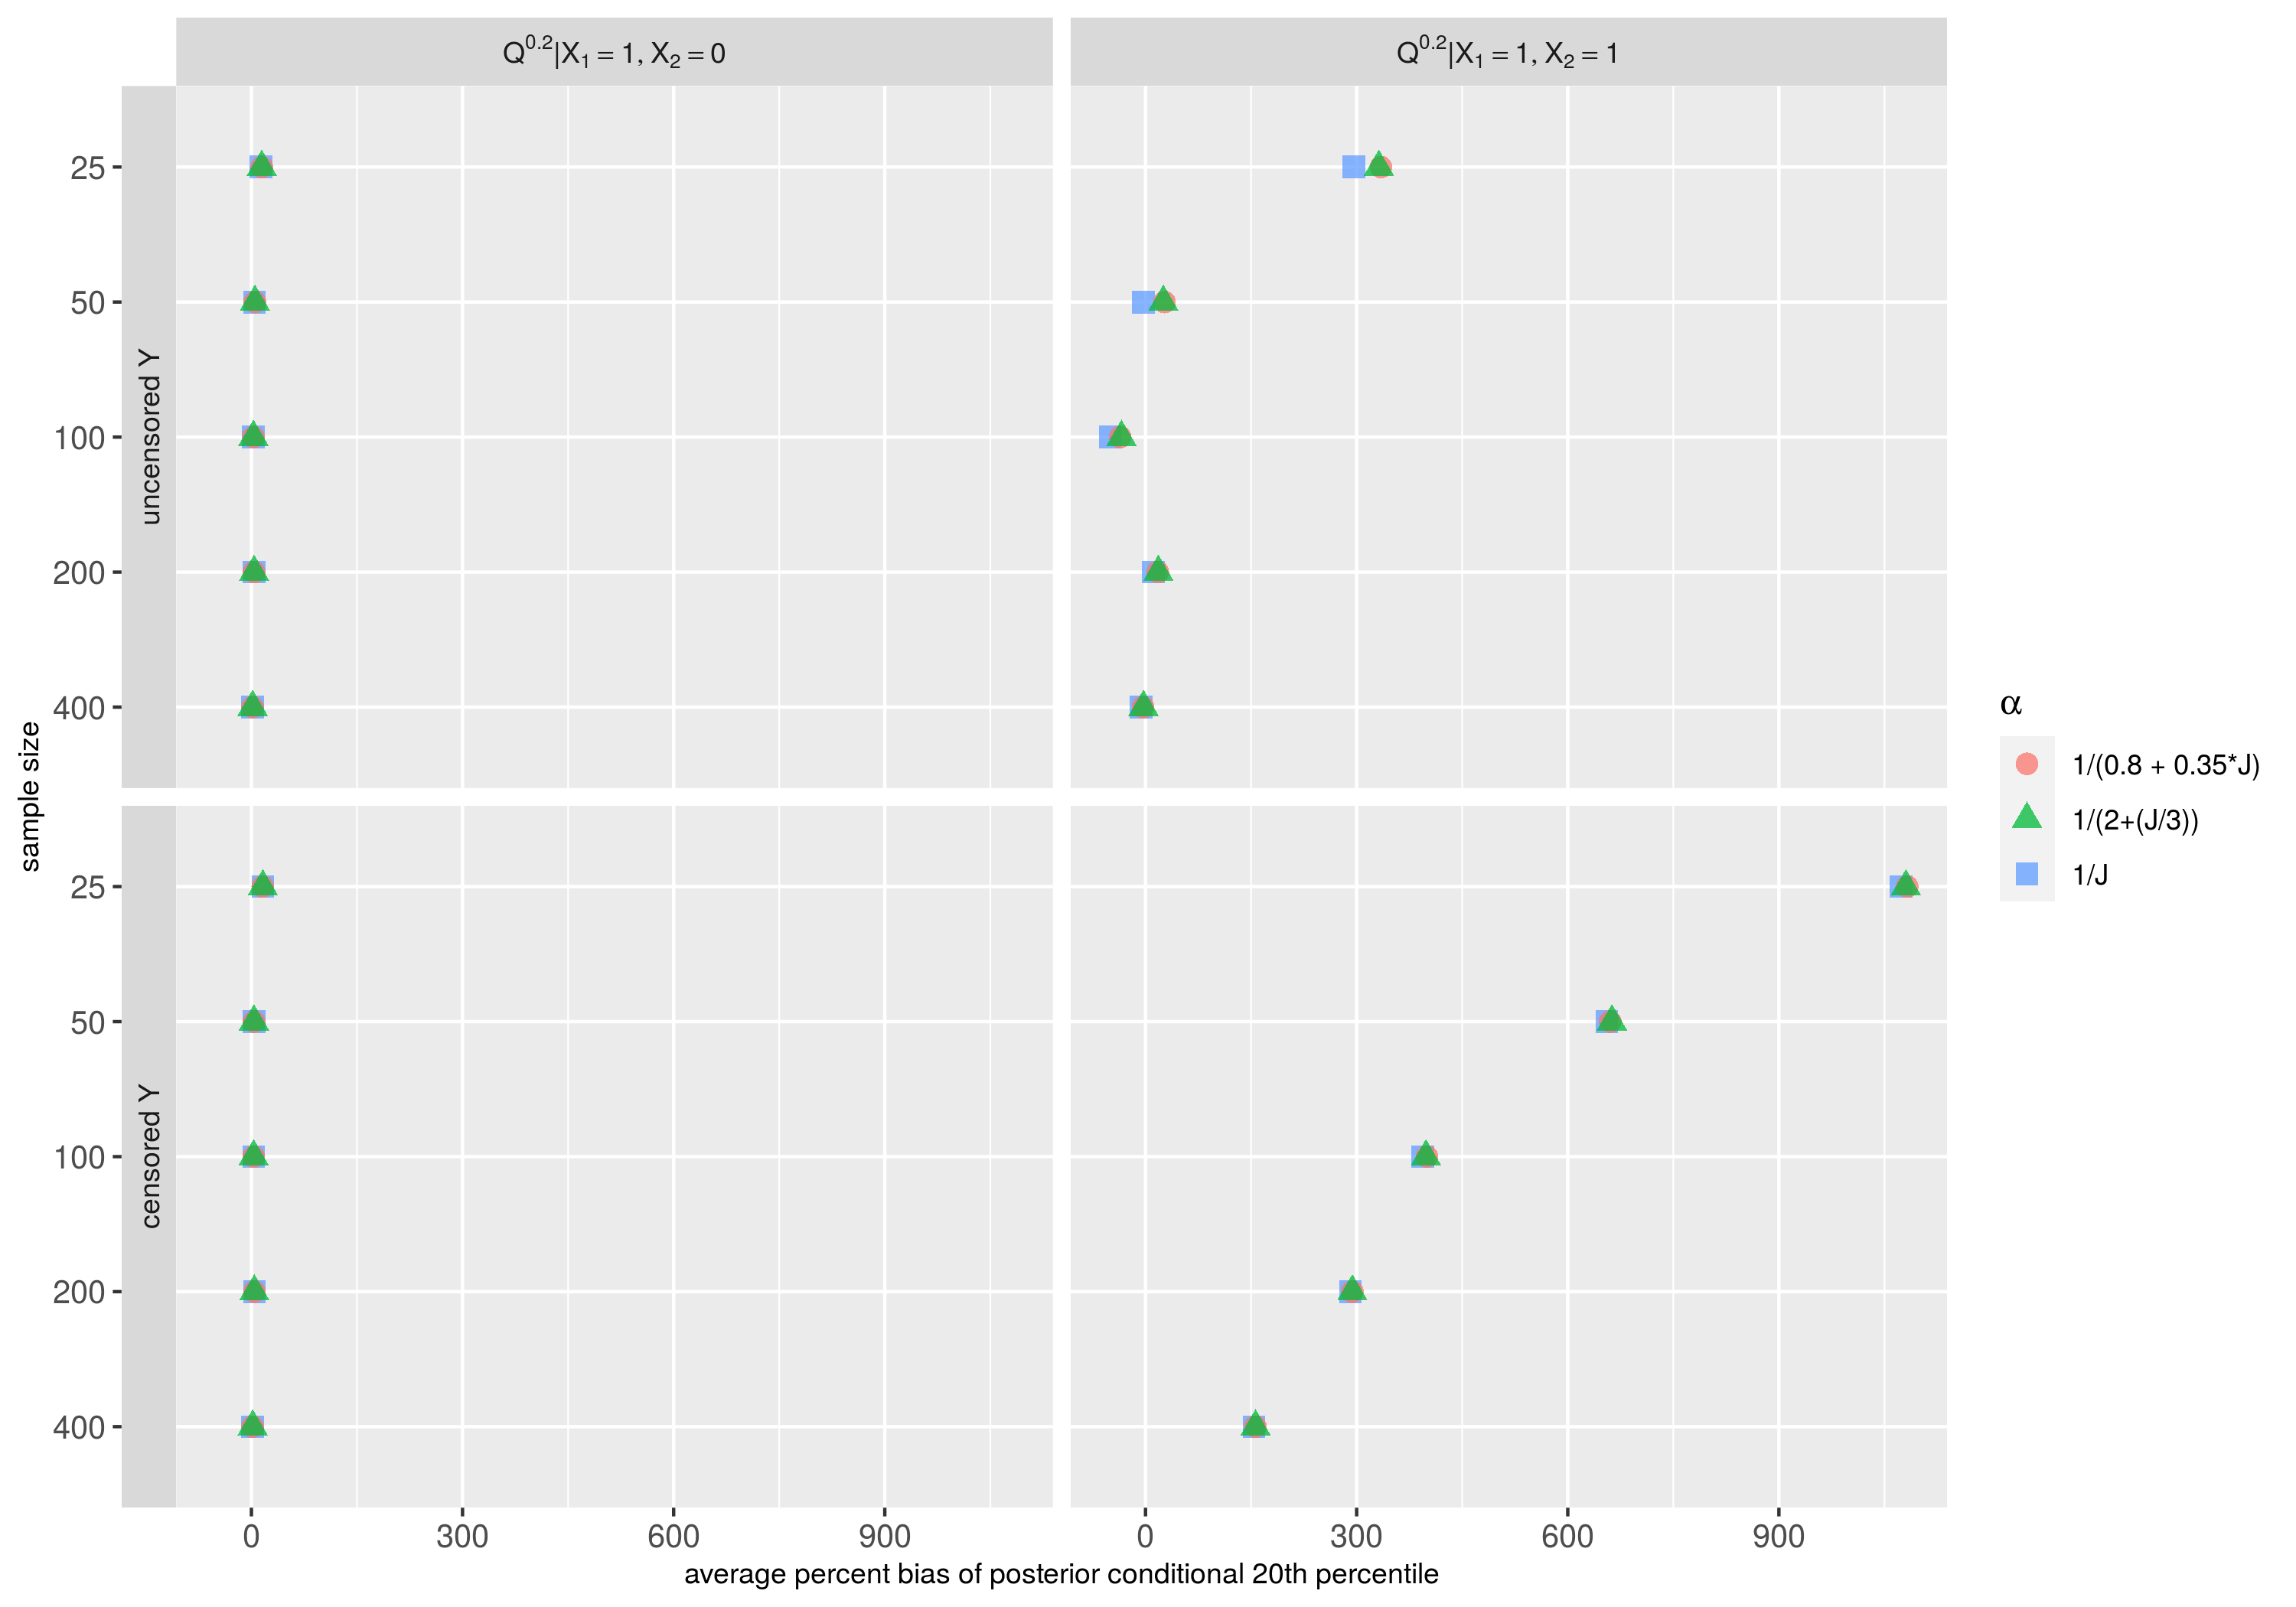
\includegraphics[width=0.75\linewidth]{fig/sim_d_q20} 

}
\caption{Bias in conditional 20th percentile for simulations using loglog link}
\end{figure}


\end{document}
